\documentclass{article}
\usepackage{iclr2024_conference,times}

\usepackage{graphicx}
\usepackage{booktabs}
\usepackage{amsmath}
\usepackage{amssymb}
\usepackage{caption}
\usepackage{subcaption}
\usepackage{hyperref}
\usepackage{url}
\usepackage{microtype}
\usepackage{placeins}

\graphicspath{{../results/figures/}}

\iclrfinalcopy % Uncomment for camera-ready version, but NOT for submission.

\title{Real-Data Driven Denoising Autoencoders for \\ 1D Periodic Time-Series Signals}

\author{Nikhil Pesaladinne \\
Duke University \\
\texttt{nrp37@duke.edu}
\And
Islam Tayeb \\
Duke University \\
\texttt{imt11@duke.edu}
}

\begin{document}

\maketitle
\lhead{CS 675 Project 2}

\begin{abstract}
This paper studies denoising autoencoders for 1D periodic signals. Real signals rarely come with clean targets. We address that by fitting a simple sinusoid to weekly Wikipedia pageview series and using that fit as a proxy clean signal. We fit three candidate noise models to the residuals, generate a synthetic training set from the fitted signal family, and compare a multilayer perceptron (MLP) autoencoder with a one-dimensional convolutional neural network (1D CNN) autoencoder. The CNN gives the best synthetic result at 15.18 dB signal-to-noise ratio (SNR) improvement with 53{,}313 parameters, versus 14.49 dB for the MLP with 101{,}136 parameters. The same CNN gives 8.91 to 11.93 dB improvement on a controlled per-article sine recovery test at the fitted Gaussian noise level ($\sigma = 0.380$ in log-pageview space). On the raw Wikipedia series it gives 2.27 to 8.06 dB improvement against the fitted-sine proxy. These results show that the synthetic benchmark is strong and that the real-data result is useful but limited by the proxy target.
\end{abstract}

\section{Introduction}

A denoising autoencoder learns to recover a clean signal from a corrupted input~\citep{vincent2008}. This is a simple idea when the clean target is known. It is harder on real time-series data, where a true clean target is rarely available.

We use weekly Wikipedia pageviews as a real 1D signal source. Disease-related pages on Wikipedia show strong seasonal structure~\citep{generous2014}. That structure makes them a good fit for this project. We model each series with a single sinusoid plus offset and trend. We then treat the fitted sinusoid as a proxy clean target.

Supervised training itself uses synthetic windows sampled from the fitted signal and noise statistics, so the benchmark still has exact clean targets.

This setup lets us study three related questions. First, can a proxy clean model estimated from real data support a useful synthetic denoising benchmark. Second, under that benchmark, how do a multilayer perceptron autoencoder and a one-dimensional convolutional autoencoder compare in accuracy and efficiency. Third, how robust is the selected model to changes in latent size, noise family, and noise intensity. We also ask how well it transfers back to the original Wikipedia series.

The central tradeoff is clear from the start. Synthetic data gives a true target and clean metrics. Real data is more meaningful, but the target is only a proxy. The report keeps both views.

\section{Data}

\paragraph{Source.}
We use daily pageviews from the Wikimedia REST API~\citep{wikimedia}. The five articles are \texttt{Influenza}, \texttt{Common\_cold}, \texttt{Fever}, \texttt{Cough}, and \texttt{Christmas}. We freeze the date range at 2018-01-01 to 2026-04-20 for reproducibility. We resample the daily counts to weekly totals. Each series has 472 weekly points.

\paragraph{Why these articles.}
The four health-related pages show a clear yearly pattern tied to flu season. \texttt{Christmas} is a positive control. Its yearly peak is large and regular. If the pipeline cannot recover that pattern, the method is not working.

\paragraph{Transform.}
All downstream processing uses $y = \log(1 + \mathrm{pageviews})$. This reduces the scale gap across articles. It also makes the dominant yearly pattern closer to a sine wave.

\section{Method}

\subsection{Proxy Clean Signal}

For each article, we fit
\begin{equation}
\hat{y}[t] = c + m\,t + A \sin(2 \pi f\,t + \phi).
\end{equation}
We initialize the frequency with a Hanning-windowed fast Fourier transform (FFT). We then refine all parameters with bounded least squares. The fitted curve is our proxy clean signal. The residual is $r[t] = y[t] - \hat{y}[t]$.

Table~\ref{tab:sinefits} shows the fitted periods and coefficient-of-determination values ($R^2$). Four articles land near the expected one-year period. \texttt{Cough} is the exception. Its fitted period is about 301 weeks, so its proxy target is weaker than the others.

\begin{table}[t]
\centering
\caption{Per-article sine-fit summary in log space.}
\label{tab:sinefits}
\begin{tabular}{lrrr}
\toprule
Article & Period (weeks) & $R^2$ & Amplitude \\
\midrule
Influenza    & 51.3  & 0.633 & 0.380 \\
Common\_cold & 51.1  & 0.589 & 0.307 \\
Fever        & 50.9  & 0.776 & 0.136 \\
Cough        & 300.9 & 0.570 & 0.186 \\
Christmas    & 52.1  & 0.554 & 0.897 \\
\bottomrule
\end{tabular}
\end{table}

\begin{figure}[t]
\centering
\begin{subfigure}{0.49\linewidth}
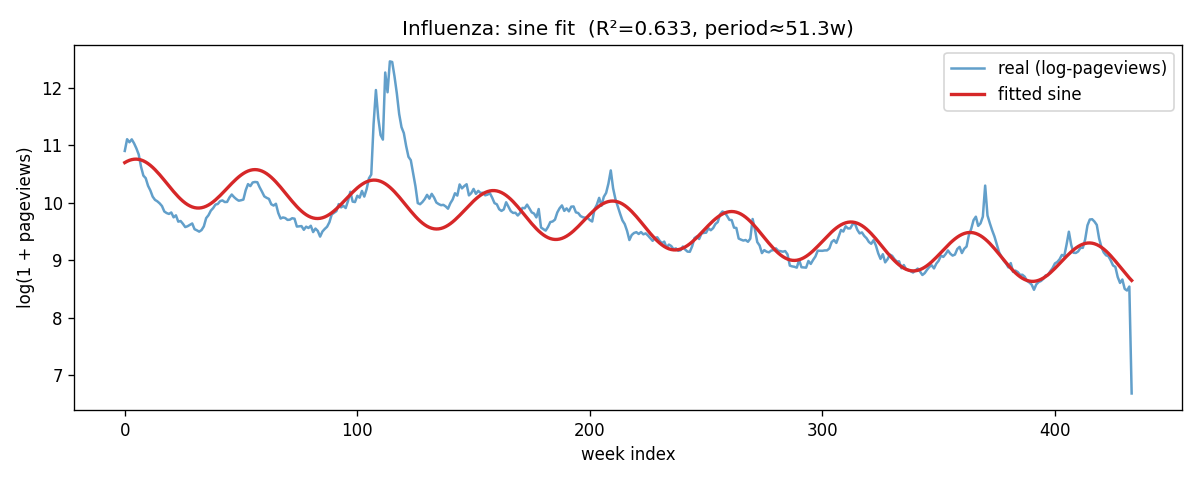
\includegraphics[width=\linewidth]{exp_1_fit/Influenza_sine_fit.png}
\caption{Influenza.}
\end{subfigure}
\hfill
\begin{subfigure}{0.49\linewidth}
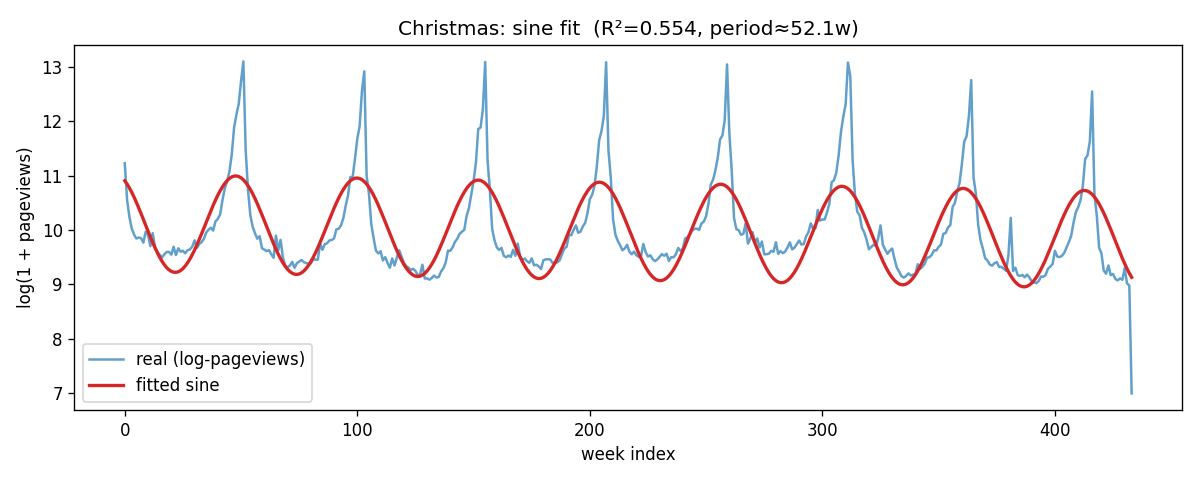
\includegraphics[width=\linewidth]{exp_1_fit/Christmas_sine_fit.png}
\caption{Christmas.}
\end{subfigure}
\caption{Example sine fits in log space. The global fit captures the annual cycle, but it misses some year-to-year amplitude change.}
\label{fig:sinefits}
\end{figure}

\subsection{Residuals And Noise Models}

We pool residuals across articles and fit three candidate noise models.
\begin{itemize}
  \item \textbf{Gaussian noise:} additive zero-mean noise with standard deviation $\sigma$.
  \item \textbf{Masking noise:} short contiguous segments are replaced by the local mean.
  \item \textbf{Impulse noise:} sparse spikes are added at random indices.
\end{itemize}

We score each fitted noise model against the observed residuals. The main score is Wasserstein distance. We also report the Kolmogorov-Smirnov statistic, the kurtosis gap, and the standard-deviation ratio. Lower Wasserstein is better.

\subsection{Synthetic Dataset}

We turn the fitted real-data parameters into a synthetic signal family. We sample offsets, slopes, amplitudes, frequencies, and phases from the fitted ranges. Each clean window has length 128. We z-score each clean window. We then corrupt it with one fitted noise model.

Each training split uses 8000 train windows, 1000 validation windows, and 1000 test windows. This gives a true clean target for every synthetic sample. That makes mean squared error (MSE) and signal-to-noise ratio (SNR) easy to interpret.

\subsection{Models, Training, And Metrics}

We compare two models.
\begin{itemize}
  \item \textbf{MLP autoencoder:} $128 \rightarrow 256 \rightarrow 64 \rightarrow z \rightarrow 64 \rightarrow 256 \rightarrow 128$.
  \item \textbf{1D CNN autoencoder:} encoder channels $1 \rightarrow 16 \rightarrow 32 \rightarrow 64$ with kernel sizes 7, 5, and 3 and stride 2. The decoder mirrors this stack with transposed convolutions.
\end{itemize}

We train with mean squared error, Adam, learning rate $10^{-3}$, batch size 64, and early stopping. The default latent size is $z=16$ unless noted otherwise.

We report
\begin{gather}
\mathrm{MSE}(x, \hat{x}) = \frac{1}{NL}\sum_{n,t}(x_n[t]-\hat{x}_n[t])^2, \\
\mathrm{SNR}_{\mathrm{dB}}(x, \hat{x}) = 10\log_{10}\left(\frac{\|x\|_2^2}{\|x-\hat{x}\|_2^2}\right), \\
\Delta\mathrm{SNR} = \mathrm{SNR}_{\mathrm{dB}}(x, \hat{x}) - \mathrm{SNR}_{\mathrm{dB}}(x, x_{\mathrm{noisy}}).
\end{gather}

\section{Experiments And Results}

\subsection{Exp 2: Noise Model Selection}

Table~\ref{tab:noise} shows the fitted noise scores. Gaussian noise is the best match by Wasserstein distance. It also matches the residual standard deviation almost exactly; the fitted Gaussian standard deviation on the pooled residuals is $\sigma = 0.380$ in log-pageview space. The main weakness is tail fit. The real residuals are more heavy-tailed than a Gaussian.

\begin{table}[t]
\centering
\caption{Noise-model selection on pooled residuals. Lower Wasserstein is better.}
\label{tab:noise}
\begin{tabular}{lrrrr}
\toprule
Kind & Wasserstein & Kolmogorov-Smirnov & Kurtosis diff & Std ratio \\
\midrule
Gaussian & \textbf{0.106} & \textbf{0.118} & -10.06 & 0.999 \\
Masking  & 0.241          & 0.569          & 819.49 & 0.111 \\
Impulse  & 0.275          & 0.559          & 48.97  & 1.908 \\
\bottomrule
\end{tabular}
\end{table}

\begin{figure}[t]
\centering
\begin{subfigure}{0.58\linewidth}
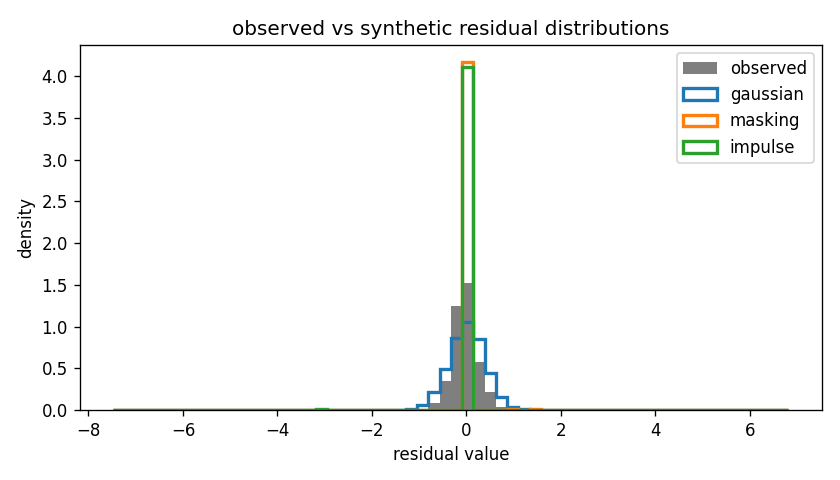
\includegraphics[width=\linewidth,trim=0.2in 0.15in 0.2in 0.15in,clip]{exp_2_noise_select/residual_hist_overlay.png}
\caption{Residual histogram overlay.}
\end{subfigure}
\hfill
\begin{subfigure}{0.38\linewidth}
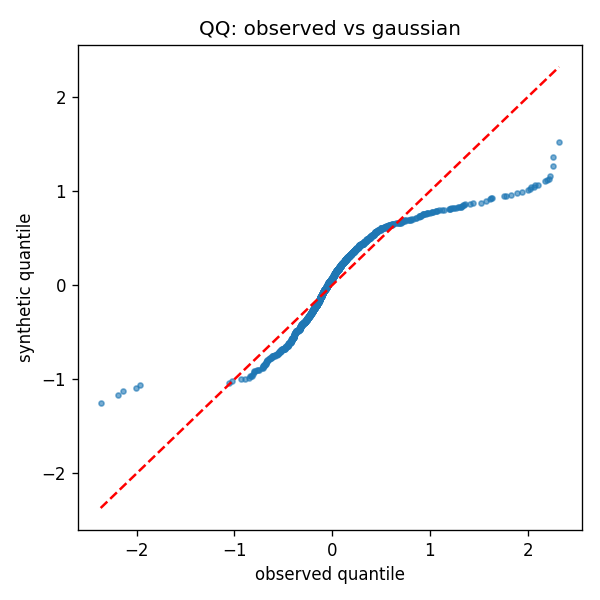
\includegraphics[width=\linewidth,trim=0.15in 0.15in 0.15in 0.15in,clip]{exp_2_noise_select/qq_gaussian.png}
\caption{Gaussian Q-Q plot.}
\end{subfigure}
\caption{Residual fit diagnostics. Left: Gaussian matches the center of the distribution well; masking and impulse are visibly more distorted. Right: the center tracks the diagonal, but the tails bend away, which shows the residuals are more heavy-tailed than a Gaussian.}
\label{fig:noise-diag}
\end{figure}

\subsection{Exp 3: Architecture Comparison}

Table~\ref{tab:arch} compares the MLP and the 1D CNN on the synthetic benchmark. The 1D CNN is better on every main test metric. It improves SNR by 15.18 dB. The MLP improves SNR by 14.49 dB. The CNN also uses about half as many parameters. The price is training time. The CNN is much slower to train.

\begin{table}[t]
\centering
\caption{Architecture comparison on the synthetic test set.}
\label{tab:arch}
\begin{tabular}{lrrrrr}
\toprule
Model & Params & Test MSE & Output SNR & $\Delta$SNR & Train (s) \\
\midrule
MLP   & 101{,}136          & 0.00632          & 22.95          & 14.49          & 56.8  \\
CNN1D & \textbf{53{,}313}  & \textbf{0.00525} & \textbf{23.63} & \textbf{15.18} & 585.7 \\
\bottomrule
\end{tabular}
\end{table}

\begin{figure}[t]
\centering

\includegraphics[width=0.75\linewidth]{exp_3_arch/training_curves.png}
\caption{Training and validation loss for the architecture comparison. Both models converge cleanly. The CNN reaches the lower final validation loss.}
\label{fig:training}
\end{figure}

\subsection{Exp 4: Latent Dimension Sweep}

Table~\ref{tab:latent} shows the latent sweep for the CNN. The big jump is from latent 4 to latent 8. The best test MSE is at latent 16. Latent 32 gives almost the same SNR improvement, but it is larger. We use latent 16 for the rest of the report.

\begin{table}[t]
\centering
\caption{Latent sweep for the 1D CNN.}
\label{tab:latent}
\begin{tabular}{rrrr}
\toprule
Latent & Params & Test MSE & $\Delta$SNR \\
\midrule
 4 & 28{,}725          & 0.01407          & 11.56 \\
 8 & 36{,}921          & 0.00559          & 14.91 \\
16 & 53{,}313          & \textbf{0.00527} & 15.17 \\
32 & 86{,}097          & 0.00535          & \textbf{15.19} \\
64 & 151{,}665         & 0.00534          & 15.16 \\
\bottomrule
\end{tabular}
\end{table}

\subsection{Exp 5 And Exp 6: Robustness To Noise Type And Noise Level}

Cross-noise robustness shows a clear diagonal pattern. Each model works best on the same noise type it saw in training. The masking-trained and impulse-trained models do very well on matched noise, at 25.17 dB and 24.55 dB respectively. Their transfer is weaker. The worst case is masking-trained on impulse noise at $-2.14$ dB. The Gaussian-trained model is the most balanced. It gets 15.13 dB on Gaussian, 11.07 dB on masking, and 9.74 dB on impulse.

Noise-level generalization is also strong. The CNN is trained at the fitted Gaussian level ($\sigma = 0.380$). From $0.75\times$ to $3.0\times$ that level, SNR improvement stays between 14.34 and 15.73 dB. Performance drops at $0.25\times$ because the input is already much cleaner.

\begin{figure}[t]
\centering
\begin{subfigure}{0.48\linewidth}
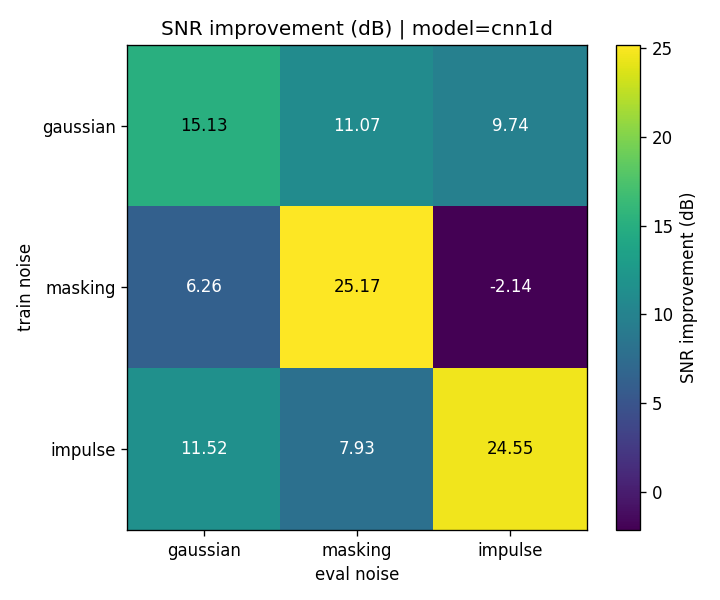
\includegraphics[width=\linewidth]{exp_5_noise_robustness/robustness_heatmap.png}
\caption{Cross-noise robustness.}
\end{subfigure}
\hfill
\begin{subfigure}{0.48\linewidth}
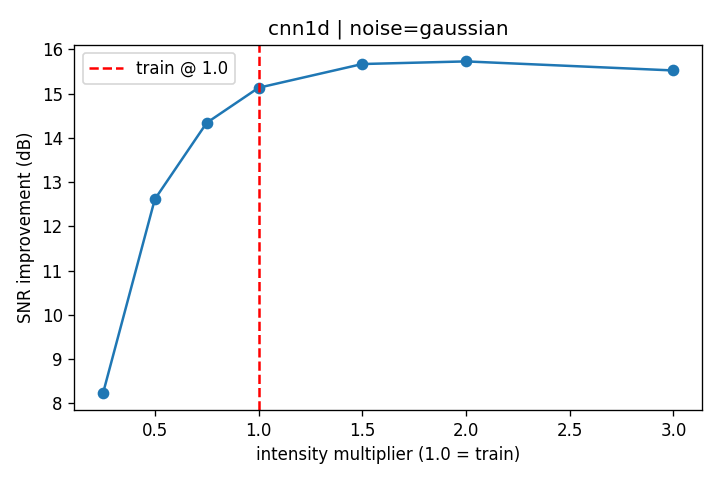
\includegraphics[width=\linewidth]{exp_6_noise_levels/snr_imp_vs_intensity.png}
\caption{Noise-level generalization.}
\end{subfigure}
\caption{Generalization results for noise type and noise level. The left panel shows strong diagonal dominance. The right panel shows stable performance from $0.75\times$ to $3.0\times$ noise.}
\label{fig:generalization}
\end{figure}

\subsection{Exp 7: Raw Wikipedia Evaluation}

This experiment works directly on the raw Wikipedia series. We slide 128-week windows with stride 1. We z-score each window, denoise it, undo the z-score, and overlap-average the window outputs back into one full series.

We then compare the reconstruction to the fitted sine proxy. Table~\ref{tab:real-eval} shows the results. Improvement ranges from 2.27 to 8.06 dB. \texttt{Christmas} is the strongest case. \texttt{Cough} is the weakest. That is consistent with the earlier fit quality.

\begin{table}[t]
\centering
\caption{Raw Wikipedia evaluation against the fitted-sine proxy.}
\label{tab:real-eval}
\begin{tabular}{lrrrr}
\toprule
Article & MSE vs fitted sine & Reconstruction SNR & Raw-series SNR & $\Delta$SNR \\
\midrule
Influenza    & 0.0855 & 30.37          & 27.74 & 2.63          \\
Common\_cold & 0.0656 & 31.06          & 28.41 & 2.65          \\
Fever        & 0.0160 & 37.12          & 32.96 & 4.16          \\
Cough        & 0.0493 & 30.99          & 28.72 & 2.27          \\
Christmas    & 0.0502 & \textbf{32.99} & 24.94 & \textbf{8.06} \\
\bottomrule
\end{tabular}
\end{table}

\subsection{Exp 8: Controlled Per-Article Sine Recovery}

This experiment is the closest real-data match to the synthetic task. For each article, we take its fitted sine as the clean target. We add Gaussian noise at the fitted level ($\sigma = 0.380$). We then denoise it with the trained CNN. The mean improvement is 10.07 dB. The range is 8.91 to 11.93 dB.

The clean-pass SNR is also strong. When we feed the clean fitted sine into the autoencoder, the mean SNR is 65.46 dB. That tells us the model adds very little distortion when the input is already clean.

\begin{table}[t]
\centering
\caption{Per-article sine recovery at the fitted Gaussian noise level ($\sigma = 0.380$).}
\label{tab:sine-recovery}
\small
\begin{tabular}{lrrrrr}
\toprule
Article & Reconstruction MSE & Input SNR & Reconstruction SNR & $\Delta$SNR & Clean-pass SNR \\
\midrule
Influenza    & 0.0138          & 28.07          & 38.37          & 10.30          & 64.77 \\
Common\_cold & 0.0150          & 27.61          & 37.55          & 9.94           & 66.49 \\
Fever        & 0.0174          & 27.53          & 36.80          & 9.26           & 68.43 \\
Cough        & 0.0190          & 26.30          & 35.21          & 8.91           & 71.19 \\
Christmas    & \textbf{0.0095} & 28.38          & \textbf{40.31} & \textbf{11.93} & 56.44 \\
\midrule
Mean         & 0.0149          & 27.58          & 37.65          & 10.07          & 65.46 \\
\bottomrule
\end{tabular}
\end{table}

The intensity sweep is stable here too. Across all five articles, the improvement stays positive across the full $0.25\times$ to $3.0\times$ range. At $3.0\times$ noise, every article still gets at least 8.82 dB improvement.

\begin{figure}[t]
\centering
\begin{subfigure}{0.49\linewidth}
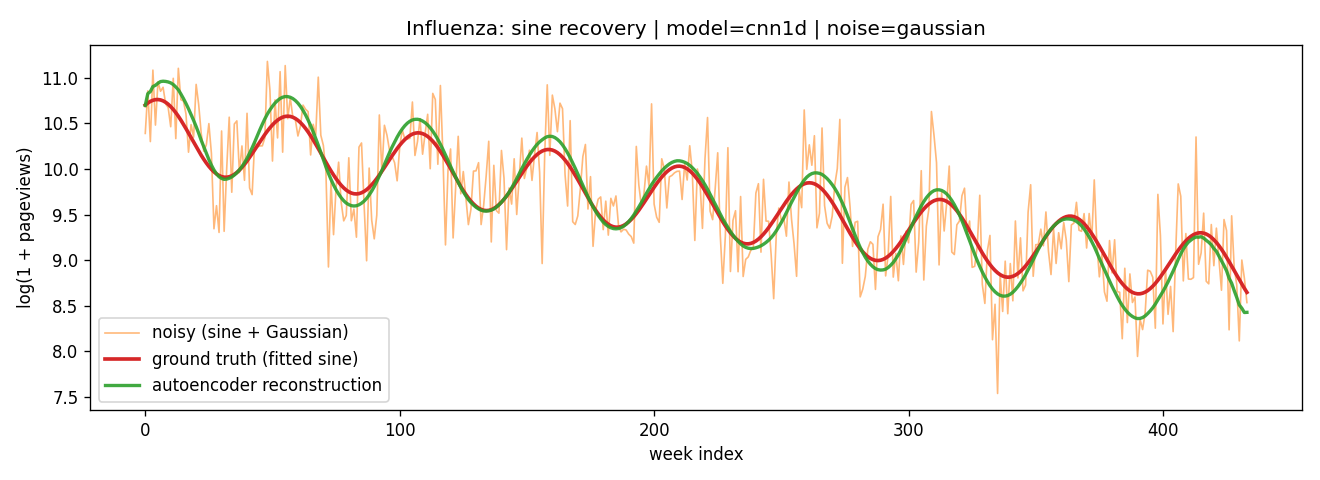
\includegraphics[width=\linewidth]{exp_8_sine_recovery/Influenza_sine_recovery.png}
\caption{Controlled sine recovery (Exp 8).}
\end{subfigure}
\hfill
\begin{subfigure}{0.49\linewidth}
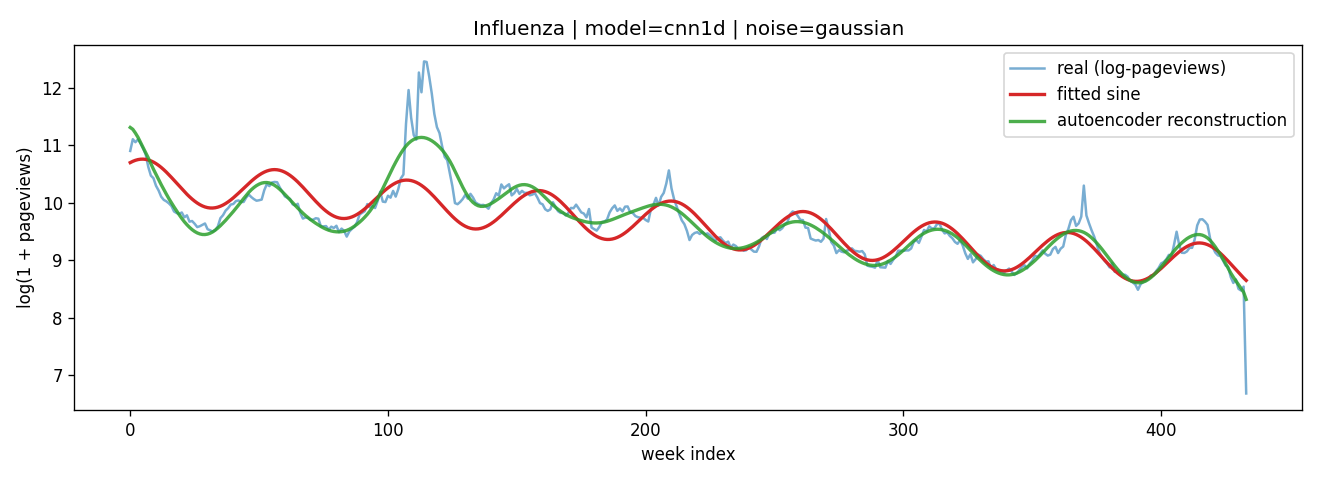
\includegraphics[width=\linewidth]{exp_7_real_eval/Influenza_real_eval.png}
\caption{Raw Wikipedia evaluation (Exp 7).}
\end{subfigure}
\caption{Two views of real-data behavior for \texttt{Influenza}. The left panel matches the synthetic task closely. The right panel shows the harder raw-series setting.}
\label{fig:real}
\end{figure}

\FloatBarrier

\section{Discussion}

The synthetic benchmark gives the clearest performance signal. It has a known target. It also matches the way the models are trained. Under that setup, the 1D CNN is the best model we tested.

The raw Wikipedia result is smaller for a clear reason. The fitted sine is only a proxy target. The denoised series can follow real nonstationary structure, such as changing seasonal amplitude, and still look worse against one global sine. That is why Exp 7 and Exp 8 should not be read as the same metric.

\texttt{Cough} is the main edge case. Its fitted period is far from one year. That weakens both the synthetic signal family and the proxy target for raw evaluation. The model still helps, but the interpretation is less clean.

The noise model is another limitation. Gaussian noise wins among the three tested families, but it does not match the residual tails well. A broader noise family could improve realism. The clean signal family is also narrow. It uses one dominant sinusoid plus a linear trend. A richer family could capture more local structure.

\section{Conclusion}

We built an end-to-end denoising autoencoder pipeline for 1D periodic signals. We grounded the synthetic benchmark in statistics from a real dataset. The 1D CNN gave the best synthetic result, the best final model, and stable performance across noise types and levels. It also gave useful gains on two real-data evaluations.

The main caveat is the proxy clean target. On real data, the fitted sine is only an approximation. Even so, the pipeline gives a consistent picture. The synthetic benchmark is strong, the controlled sine recovery test is also strong, and the raw-series result is positive but more conservative.

Code and report files are available at \url{https://github.com/IslamTayeb/denoise-autoencoder}.

\subsubsection*{Acknowledgements}

Both authors, Nikhil Pesaladinne and Islam Tayeb, contributed jointly to the code and the report. We used Claude Code to assist with writing the implementations.

\bibliography{iclr2024_conference}
\bibliographystyle{iclr2024_conference}

\end{document}
